% ------------ LSA-proceedings-template.tex  -- LSA proceedings template ---------------------------------------------------------------------------
% created by Sarah E. Murray, 24 April 2017 based on the LSA's stylesheet
% http://journals.linguisticsociety.org/proceedings/index.php/PLSA/pages/view/instructions
%Updated by Patrick Farrell, February 1, 2019.
%
% ------------ begin preamble -----------------------------------------------------------------------------------------
 \documentclass[12pt,letterpaper]{article}	
% ------------ personal packages ----------------------------------------------------------------------------
\usepackage{linguex}	%http://texdoc.net/texmf-dist/doc/latex/linguex/linguex-doc.pdf
% ------------ LSA page layout and packages ----------------------------------------------------------------------------
\usepackage{times}
\usepackage{natbib}
 	\setcitestyle{semicolon,aysep={},yysep={,},notesep={; }}
\usepackage{lipsum}          % this and the following package and the settings beneath them are for maintaining indentation and still having ragged-right aligmnent
\usepackage{ragged2e}
\setlength\RaggedRightParindent{0.3in}
\RaggedRight

\usepackage{graphicx}
\usepackage{booktabs}
\usepackage{amssymb} % checkmark
\usepackage[normalem]{ulem}
\usepackage{qtree}
\qtreecenterfalse
\newcommand{\sem}[1]{\mbox{$[\![$#1$]\!]$}}
\newcommand{\lam}{$\lambda$}
\newcommand{\lan}{$\langle$}
\newcommand{\ran}{$\rangle$}
\newcommand{\type}[1]{\ensuremath{\left \langle #1 \right \rangle }}
\renewcommand{\firstrefdash}{}

\usepackage{fullpage} 
\usepackage[compact]{titlesec}
	\titleformat{\section}[runin]{\normalfont\bfseries}{\thesection.}{.5em}{}[.]
	\titleformat{\subsection}[runin]{\normalfont\scshape}{\thesubsection}{.5em}{}[.]
\usepackage[usenames,dvipsnames]{color}	
\usepackage[colorlinks,allcolors={black},urlcolor={blue}]{hyperref} 		%likes to be last package 
% -------------- personal definitions ---------------------------------------------------------------------------------------------------------   
% -------------- LSA definitions ---------------------------------------------------------------------------------------------------------           
\setlength\parindent{0.3in}			%paragraphs indented 0.3inches
\setlength\intextsep{6pt}			%spacing before and after tables
\setlength\abovecaptionskip{6pt}	%spacing between figure and caption
%-------------------------------------------------------------- format title --------------------------------------
\makeatletter
\def\@maketitle{%
  \newpage
  \begin{center}%
  \let \footnote \thanks
    {\normalfont\bfseries \@title \par}%
    {\vskip .5em%\vskip 6pt%
      \begin{tabular}[t]{c}%
        \@author
      \end{tabular}\par}%
  \end{center}%
  \par}
\makeatother
%-------------------------------------------------------------- format abstract environment --------------------------------------
% Abstracts have to be 12pt, indented 1.4 inches on each side, and inline with the label
\renewenvironment{abstract}{%
\noindent\begin{minipage}{1\textwidth}
\setlength{\leftskip}{0.4in}
\setlength{\rightskip}{0.4in}
\textbf{Abstract.}}
{\end{minipage}}
%-------------------------------------------------------------- format keywords environment --------------------------------------
% Abstracts have to be 12pt, indented 1.4 inches on each side, and inline with the 
\newenvironment{keywords}{%
\vspace{.5em}
\noindent\begin{minipage}{1\textwidth}
\setlength{\leftskip}{0.4in}
\setlength{\rightskip}{0.4in}
\textbf{Keywords.}}
{\end{minipage}}
%-------------------------------------------------------------- title information --------------------------------------%
\title{
	On the role of conjunction in adjective ordering preferences
} 
%
\author{Cesar Manuel Rosales Jr.~\& Gregory Scontras\footnote{
		Authors: Cesar Manuel Rosales Jr., University of California, Irvine (\href{mailto:CESARMR@uci.edu}{cesarmr@uci.edu}),
		Gregory Scontras, University of California, Irvine (\href{mailto:g.scontras@uci.edu}{g.scontras@uci.edu}).
	}
}
% ------------ end preamble ------------------------------------------------------------------------------------------------
% 
%
%
% ------------ begin main document --------------------------------------------------------------------------------------
 
 
\begin{document} 

%%If using linguex, need the following commands to get correct LSA style spacing
%% these have to be after  \begin{document}
\setlength{\Extopsep}{6pt}
\setlength{\Exlabelsep}{9pt}		%effect of 0.4in indent from left text edge
%%
 
\maketitle

\begin{abstract}
	Adjective ordering preferences are robustly attested in English and many unrelated languages. In nominals with multi-adjective strings (e.g., \emph{big blue box}), chances are the order of the adjectives is non-arbitrary. However, ordering preferences are claimed to neutralize in cases where multi-adjective strings are formed via conjunction (e.g., \emph{blue \uline{and} big box}). We provide empirical evidence in support of this claim, but with an important caveat: conjunction neutralizes adjective ordering preferences in languages like Spanish where multi-adjective strings obligatorily feature conjunction. In English, where multi-adjective strings optionally feature conjunction, ordering preferences persist in the presence of conjunction.
\end{abstract}

\begin{keywords}
	adjective ordering; subjectivity; conjunction; Spanish
\end{keywords}

\section{Introduction}

In cases of adjectival modification, speakers are not limited to using a single adjective. We may talk of big blue boxes or new plastic chairs. However, the relative order of the two adjectives is not arbitrary: our ordering preferences dictate that \emph{big blue box} sounds vastly more natural than the reverse order, \emph{blue big box}. Curiously, the exact same preferences have been reported in a range of diverse languages, both with pre- and post-nominal adjectives \citep[e.g., Hungarian, Dutch, Mandarin Chinese, Indonesian, Tagalog;][]{Martin1969competence,hetzron1978,dixon1982,sproatshih1991,samontescontras2019}. It would seem that these preferences attend to the relative distance of adjectives from the nouns they modify.

Recently, \cite{scontrasetal2017adjectives} used behavioral and corpus evidence to document the predictive power of adjective subjectivity in adjective ordering preferences. The authors showed that adjective order in multi-adjective strings is best predicted by the subjectivity of the adjectives involved, such that less subjective adjectives are preferred closer to the modified noun---at least in English. To the extent that other languages demonstrate the English preferences, subjectivity is likely to play a role there as well.

Recent accounts of the role of subjectivity in adjective ordering preferences demonstrate how subjectivity-based orderings maximize communicative success in the incremental construction of a noun phrase. However, these accounts split on whether they assume hierarchical semantic composition \citep{simonic2018,scontrasetalSPadjectives} or a linear, flat process \citep{hahnetal2018}. The current work explores a prediction on which these two accounts differ: conjunction disrupts the incremental hierarchical composition of multi-adjective strings, but not its linear ordering; to the extent that conjunction neutralizes ordering preferences, we will have evidence in favor of the hierarchical account. To test this prediction, we explore ordering preference in Spanish, a language with post-nominal adjectives that require conjunction in multi-adjective strings.

The paper is structured as follows. In Section \ref{background}, we survey the empirical foundations of subjectivity-based ordering preferences established by \cite{scontrasetal2017adjectives}, as well as recent proposals accounting for the role of subjectivity. In Section \ref{spanish}, we extend the original English methodology from \cite{scontrasetal2017adjectives} to determine the status of subjectivity-based ordering preferences in Spanish. We return to English in Section \ref{english}, where we test for preferences both with and without conjunction. Section \ref{discussion} concludes with a discussion of our findings.


\section{Background} \label{background}

Adjective ordering preferences have received a good deal of attention in both the linguistics and psychology literatures, and with good reason: that we should find the same preferences in such a diverse range of languages must evidence deep properties of language and the minds from which it emerges. Proposals split on whether they attempt to characterize the linguistic representation of these preferences \citep[e.g.,][]{dixon1982,cinque1994,scott2002,mcnallyboleda2004,laenzlinger2005,truswell2009} or the psychological factors that predict them \citep[e.g.,][]{Sweet1898,whorf1945,ziff1960,Martin1969competence,seiler1978}. Inspired by accounts linking ordering preferences to properties of adjective meaning, \cite{scontrasetal2017adjectives} pursued the hypothesis that adjective subjectivity predicts adjective ordering preferences \citep{quirketal1985,hetzron1978,tucker1998,hill2012}.

To test the subjectivity hypothesis, \cite{scontrasetal2017adjectives} first established a behavioral measure of English ordering preferences. They presented experimental participants with pairs of multi-adjective strings that differed in the relative order of the adjectives, and asked participants to indicate which order sounded more natural. The authors validated their behavioral measure by comparing it with naturalistic productions from corpora. Next, \citeauthor{scontrasetal2017adjectives} established a behavioral measure of adjective subjectivity, which they validated with a faultless disagreement task \citep{Kolbel2004,Barker2013,Kennedy2013,MacFarlane2014}.  When comparing their estimates of the ordering preferences with the adjective subjectivity measure, \cite{scontrasetal2017adjectives} found that subjectivity accounted for 85\% of the variance in the ordering preferences for 26 adjectives from seven different semantic classes (e.g., size, color, shape, etc.). Looking at a larger collection of 74 adjectives from 13 semantic classes, the authors found that subjectivity accounted for 61\% of the variance in ordering preferences.

With strong evidence for the role of subjectivity in adjective ordering, the task shifts next to explaining why subjectivity should play the role it does in the observed preferences. All of the explanations offered to date agree that subjectivity-based orderings maximize communicative success. However, the details of these explanations differ, as does the evidence used to support them. 

\cite{simonic2018} developed a probabilistic model of utterance selection conceived within the Rational Speech Act modeling framework \citep{frankejaeger2016,goodmanfrank2016}. The model chooses between multi-adjective strings that differ in the relative order of the adjectives (e.g., \emph{big blue box} vs.~\emph{blue big box}). To model adjective subjectivity, \citeauthor{simonic2018} assumed that a listener's semantic entry for an adjective could deviate from that of the speaker; the probability of this deviation increases with subjectivity. \citeauthor{simonic2018} further assumed that meaning composition follows the hierarchical structure of modification, as in \ref{hierarchical}, such that adjectives that occur farther from the modified noun operate over a restricted set of potential references (e.g., the set of blue boxes vs.~the set of boxes). 

\ex. \label{hierarchical}
\Tree [. \emph{big} [. \emph{blue} \emph{box} ] ]

With the goal of establishing reference---in other words, signaling a specific object to a listener---\citeauthor{simonic2018} used his utterance choice model to demonstrate how ordering adjectives with respect to decreasing subjectivity is more useful in most cases, and thus more likely to be chosen by the speaker. Communicative success is maximized by ensuring that higher-subjectivity adjectives, whose semantics might vary between speakers and listeners and therefore lead to errors in alignment, operate over the smallest set of potential referents, thereby minimizing opportunities for errors in alignment between speakers and listeners.

\cite{scontrasetalSPadjectives} offered a similar explanation for subjectivity-based ordering preferences. They modeled adjective subjectivity as the probability that a listener would incorrectly classify a possible referent (e.g., incorrectly classifying some box as blue); more subjective adjectives are more likely to lead to incorrect classifications. \citeauthor{scontrasetalSPadjectives}~further assumed that classification errors increase with the size of the set to be classified. In other words, classification precision decreases as the number of classifications increases. As with \citeauthor{simonic2018}, these assumptions lead to a higher probability of correct classifications if the most error-prone (i.e., most subjective) adjectives operate over the smallest set of potential referents, composing last in the hierarchical nominal structure. \citeauthor{scontrasetalSPadjectives}~explored over 100,000 cases of multi-adjective modification, finding that subjectivity-based ordering leads to a higher probability of correct referent classification in 93\% of those cases.

Whereas \cite{simonic2018} and \cite{scontrasetalSPadjectives} assume hierarchical meaning composition, \cite{hahnetal2018} pursued a different approach, assuming instead that listeners incrementally update their beliefs with the linear flow of words. Their model further differs from those of \citeauthor{simonic2018} and \citeauthor{scontrasetalSPadjectives}~by defining speaker utility not in terms of referential success, but rather in terms of successfully communicating subjective opinions about objects in the world. In other words, \citeauthor{hahnetal2018}~model cases of non-restrictive adjectival modification. They also treat adjective subjectivity as the potential for disagreement between speakers and listeners. However, \citeauthor{hahnetal2018}~introduce memory considerations into their model: words further in the past are more likely to be forgotten. By combining incremental linear processing with memory limitations, the authors predict that speakers will maximize their utility (i.e., maximize the probability of successfully communicating their subjective opinions) by ordering adjectives with respect to decreasing subjectivity.

To summarize, all three models demonstrate how subjectivity-based orderings maximize communicative success. The models differ in the precise details of implementing subjectivity, as well as processing considerations. For present purposes, the most salient difference among these approaches concerns the mode by which meaning gets composed. \cite{simonic2018} and \cite{scontrasetalSPadjectives} assume hierarchical meaning composition that proceeds outward from the modified noun; subjectivity-based orderings ensure that adjectives with higher subjectivity compose later, thereby operating over a restricted set of potential referents. On the other hand, \cite{hahnetal2018} assume a linear process of meaning composition; subjectivity-based orderings ensure that the most subjective adjectives are most likely to be forgotten. Both styles of approach successfully predict subjectivity-based ordering preferences, and in principle, both sorts of pressures---hierarchical and linear---could be active in the construction of multi-adjective strings. However, the two styles of approach make different predictions when it comes to conjunction.

Conjunction has been claimed to neutralize ordering preferences in English \citep[e.g.,][]{fordolson1975,byrne1979}. In effect, this neutralization leads to the acceptability of otherwise-unacceptable adjective orderings. For example, whereas \emph{blue big box} is strongly dispreferred, \emph{blue and big box} should be acceptable. When we consider why pressures for subjectivity-based orderings should dissipate in the context of conjunction, the hierarchical accounts of \cite{simonic2018} and \cite{scontrasetalSPadjectives} offer a ready explanation. To reiterate the proposed mechanism: subjectivity-based orderings maximize communicative success by ensuring that the most subjective (i.e., noisiest,  least useful) adjectives compost last, operating over the smallest set of potential referents. In cases of conjunction, as schematized in \ref{conjunction}, this situation no longer holds.

\ex. \label{conjunction}
\Tree [. [. \emph{big} [. \emph{and} \emph{blue} ] ] \emph{box} ] 

With conjunction, the adjectives no longer compose incrementally with the nominal; instead, the adjectives first conjoin together, and then the conjoined structure jointly modifies the noun. Without incremental restriction, it is no longer the case that adjectives farther from the noun will operate over a restricted set of potential referents. Thus, without incremental restriction, it is no longer possible to reduce errors in alignment between speakers and listeners by placing more subjective adjectives farther from the modified noun. Crucially, the linear processing account of \cite{hahnetal2018} makes a different prediction: adjectives farther from the noun are still more likely to be forgotten, so pressures toward subjectivity-based ordering should apply with conjunction as they do without it.

We therefore set out to test the predictions of linear vs.~hierarchical accounts of subjectivity-based ordering preferences. To do so, we first look at ordering preferences in Spanish, were multi-adjective strings require conjunction. We then turn to English, bringing behavioral data to bear on the status of adjective ordering preferences with conjunction.


\section{Experiment 1: Spanish} \label{spanish}

Spanish offers a natural testbed for teasing apart the predictions of linear vs.~hierarchical accounts of subjectivity-based ordering preferences. In Spanish, multi-adjective strings are post-nominal and require conjunction, as in \ref{spanish-order}.\footnote{Some adjectives in Spanish may occur pre-nominally. However, this strategy is not fully productive in the language. We therefore focus only on post-nominal multi-adjective strings.}

\exg. la caja grande y azul \\
the box big and blue \\
`the big and blue box' \label{spanish-order}

To determine the status of ordering preferences in Spanish, we replicated the methodology from \cite{scontrasetal2017adjectives} using Spanish translations of the English materials.

\subsection{Ordering preferences} 

First, we must determine the status of Spanish ordering preferences. To do so, we replicated the methodology of \emph{Expt.~1: Ordering preferences} from \cite{scontrasetal2017adjectives} using Spanish materials.

\paragraph{Participants.}

We recruited 224 participants through Amazon.com's Mechanical Turk crowd-sourcing service. All participants were compensated for their participation. On the basis of their responses to a post-test demographics questionnaire, we identified 48 native speakers of Spanish (30 female, 18 male; mean age: 34). These participants described themselves as having learned Spanish as their first language, and still using Spanish as their primary language at the time of testing; they also reported living in a Spanish-speaking country both before and after the age of eight. Their data were included in the analyses reported below.

\paragraph{Procedure.}

\begin{table}
	\centering
	{
		\begin{tabular}{lllllllll} \toprule
			\textbf{adjective}  & \textbf{translation} & \textbf{class} &  \textbf{adjective}  & \textbf{translation} & \textbf{class}\\ \midrule
			fresco & fresh & age & bueno & good & quality \\
			nuevo & new & age & malo & bad & quality \\
			podrido & rotten & age & cuadrado & square & shape  \\
			viejo & old & age & redondo & round & shape  \\
			amarillo & yellow & color & corto & short & size \\
			azul & blue & color & enorme & huge & size  \\
			marr\'{o}n & brown & color & grande & big & size \\
			morado & purple & color & largo & long & size \\
			rojo & red & color & min\'{u}sculo & tiny & size \\
			verde & green & color & peque\~{n}o & small & size  \\
			\textit{americano} & Mexican & nationality & duro & hard & texture \\
			\textit{espa\~{n}ol} & Spanish & nationality & liso & smooth & texture \\
			\textit{mexicano} & American & nationality & suave & soft & texture \\ \midrule
			\textbf{noun} & \textbf{translation} & \textbf{class} & \textbf{noun} & \textbf{translation} & \textbf{class}\\ \midrule
			manzana & apple & food &  escritorio & desk & furniture \\
			pl\'{a}tano & banana & food & silla & chair & furniture \\
			queso & cheese & food & sof\'{a} & couch & furniture \\
			tomate & tomato & food & televisi\'{o}n & TV & furniture \\
			zanahoria & carrot & food & ventilador & fan & furniture \\ \bottomrule
		\end{tabular}
		\caption{Spanish adjectives and nouns used in Experiment 1. Words in italics indicate cases where direct translation from the original English materials was not possible.}
		\label{spanish-materials}
	}
\end{table}

Participants were tasked with providing judgments about the naturalness of object descriptions. Participants completed a total of 26 trials. On each trial, they indicated which of two object descriptions sounded more natural. To provide their ratings, participants adjusted a slider with endpoints labeled with the competing object descriptions. Each description featured two adjectives, and the description pairs differed only in the relative order of the two adjectives (e.g., \emph{la caja grande y azul} vs.~\emph{la caja azul y grande}). Adjectives and nouns were chosen at random from the materials in Table \ref{spanish-materials}, with the constraint that each description contained adjectives from two different semantic classes. Where possible, these materials were direct translations of the English materials from \cite{scontrasetal2017adjectives}; in place of the English material adjectives (i.e., \emph{metal}, \emph{plastic}, \emph{wooden}), we substituted three nationality adjectives (i.e., \emph{americano}, \emph{espa\~{n}ol}, \emph{mexicano}).



\paragraph{Results.}

\begin{figure}
	\centering
	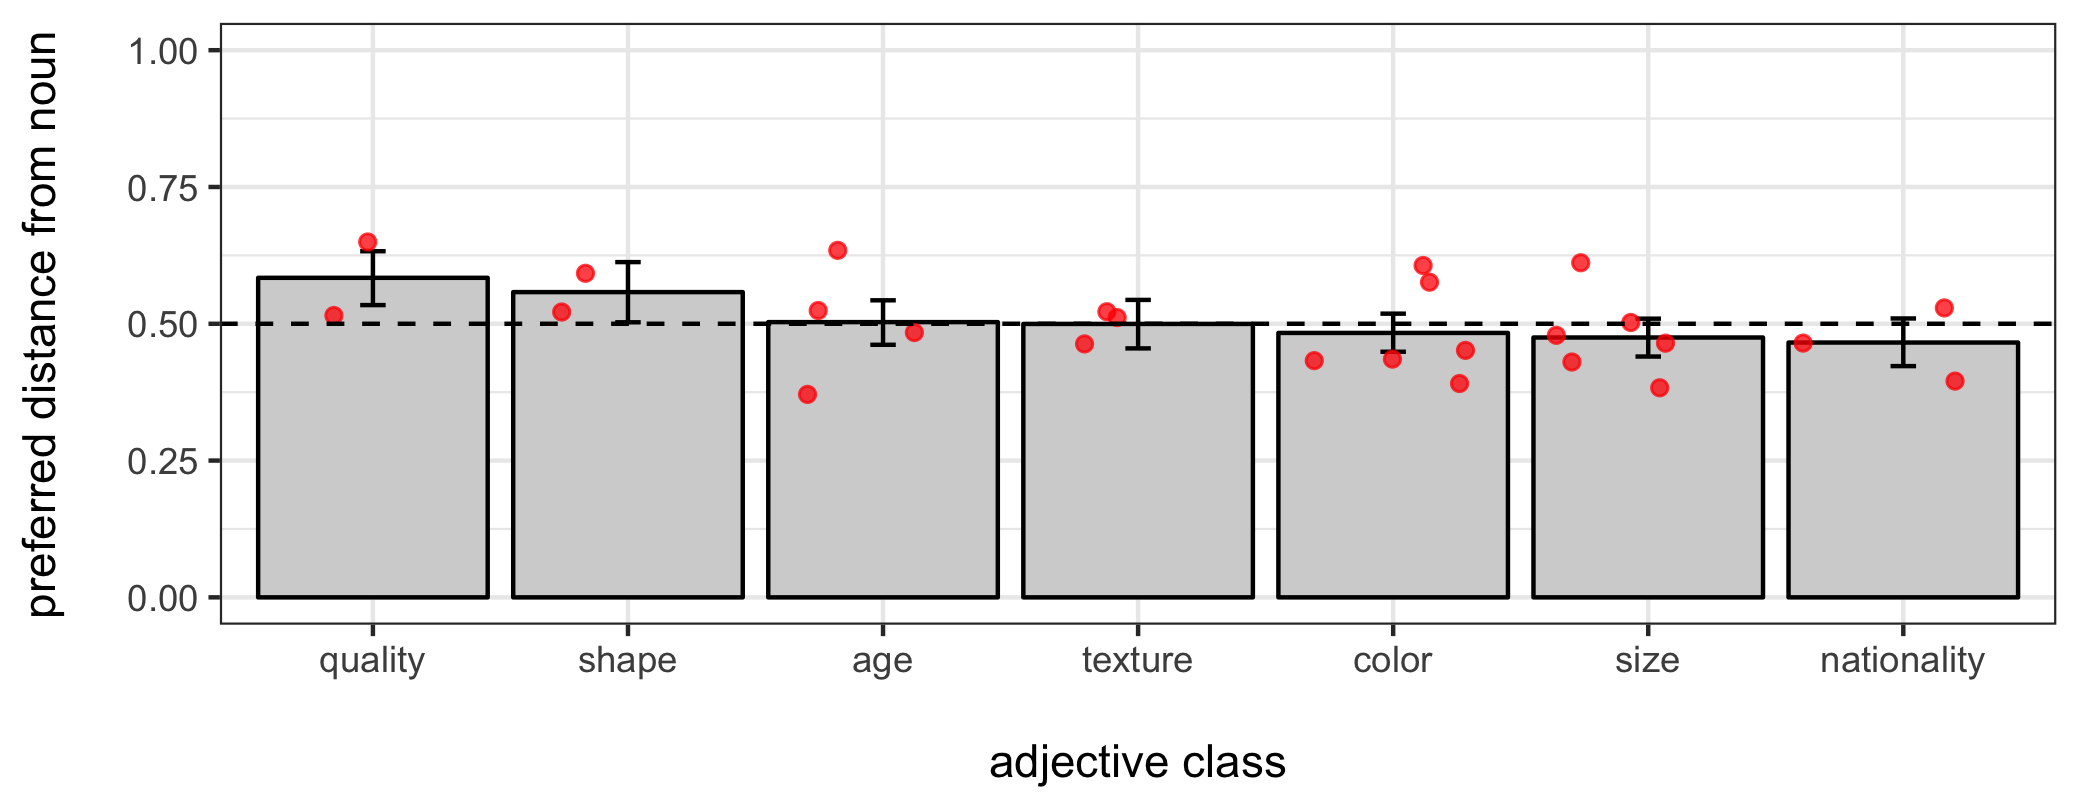
\includegraphics[height=2.5in]{class_distance_jitter.eps}
	\caption{Naturalness ratings from Experiment 1 grouped by adjective semantic class. Higher values indicate that a class's adjectives are preferred farther from the modified noun; lower values indicate that a class's adjectives are preferred closer. The dashed line indicates chance level, or the absence of stable preferences. Error bars represent bootstrapped 95\% confidence intervals drawn from 10,000 samples of the data. Red dots represent point estimates for individual adjectives.
	}
	\label{exp1-results}
\end{figure}

For each of the 26 adjectives in Table \ref{spanish-materials}, we computed a mean preferred-distance measure (i.e., how far the adjective was preferred from the modified noun) by averaging across participants. Figure \ref{exp1-results} plots these preferred distance measures grouped by adjective semantic class. There, we see that in all but one of the semantic classes (i.e., \emph{quality}), participants fail to provide systematic ratings that would evidence stable ordering preferences (i.e., a preference to place adjectives closer or farther from the modified noun); we find a similar pattern of responses at the level of individual adjectives.


\subsection{Subjectivity} 

Having documented the (absence of) ordering preferences in Spanish, we turn now to measuring Spanish adjective subjectivity. Perhaps we fail to find stable ordering preference in Spanish because participants perceive the subjectivity of the adjectives as similar. In other words, perhaps subjectivity predicts ordering preferences in Spanish as it does in English, but what differs between the two languages is the perceived subjectivity of the adjectives involved. To measure subjectivity, we replicated the methodology of \emph{Expt.~1: Faultless disagreement validation} from \cite{scontrasetal2017adjectives}. 

\paragraph{Participants.}

We recruited 106 participants who did not take part in the ordering preferences experiment through Amazon.com's Mechanical Turk. All participants were compensated for their participation. Using the same exclusion criteria from the ordering preference experiment, we identified 21 native speakers of Spanish (9 female, 12 male; mean age: 33); their data were included in the analyses reported below.


\paragraph{Procedure.}

Participants read a series of short dialogs in which two speakers disagreed about a property description for some object. For example, one speaker might assert that a box is big, while the other would disagree, saying that the box is not big. Participants judged whether both speakers could be right in their diverging statements; they adjusted a slider with endpoints labeled `no, somebody was wrong' (coded as 0) and `yes, the two may be right' (coded as 1). Participants completed a total of 26 trials, one for each of the adjectives in Table \ref{spanish-materials}.

\paragraph{Results.}

\begin{figure}[t]
	\centering
	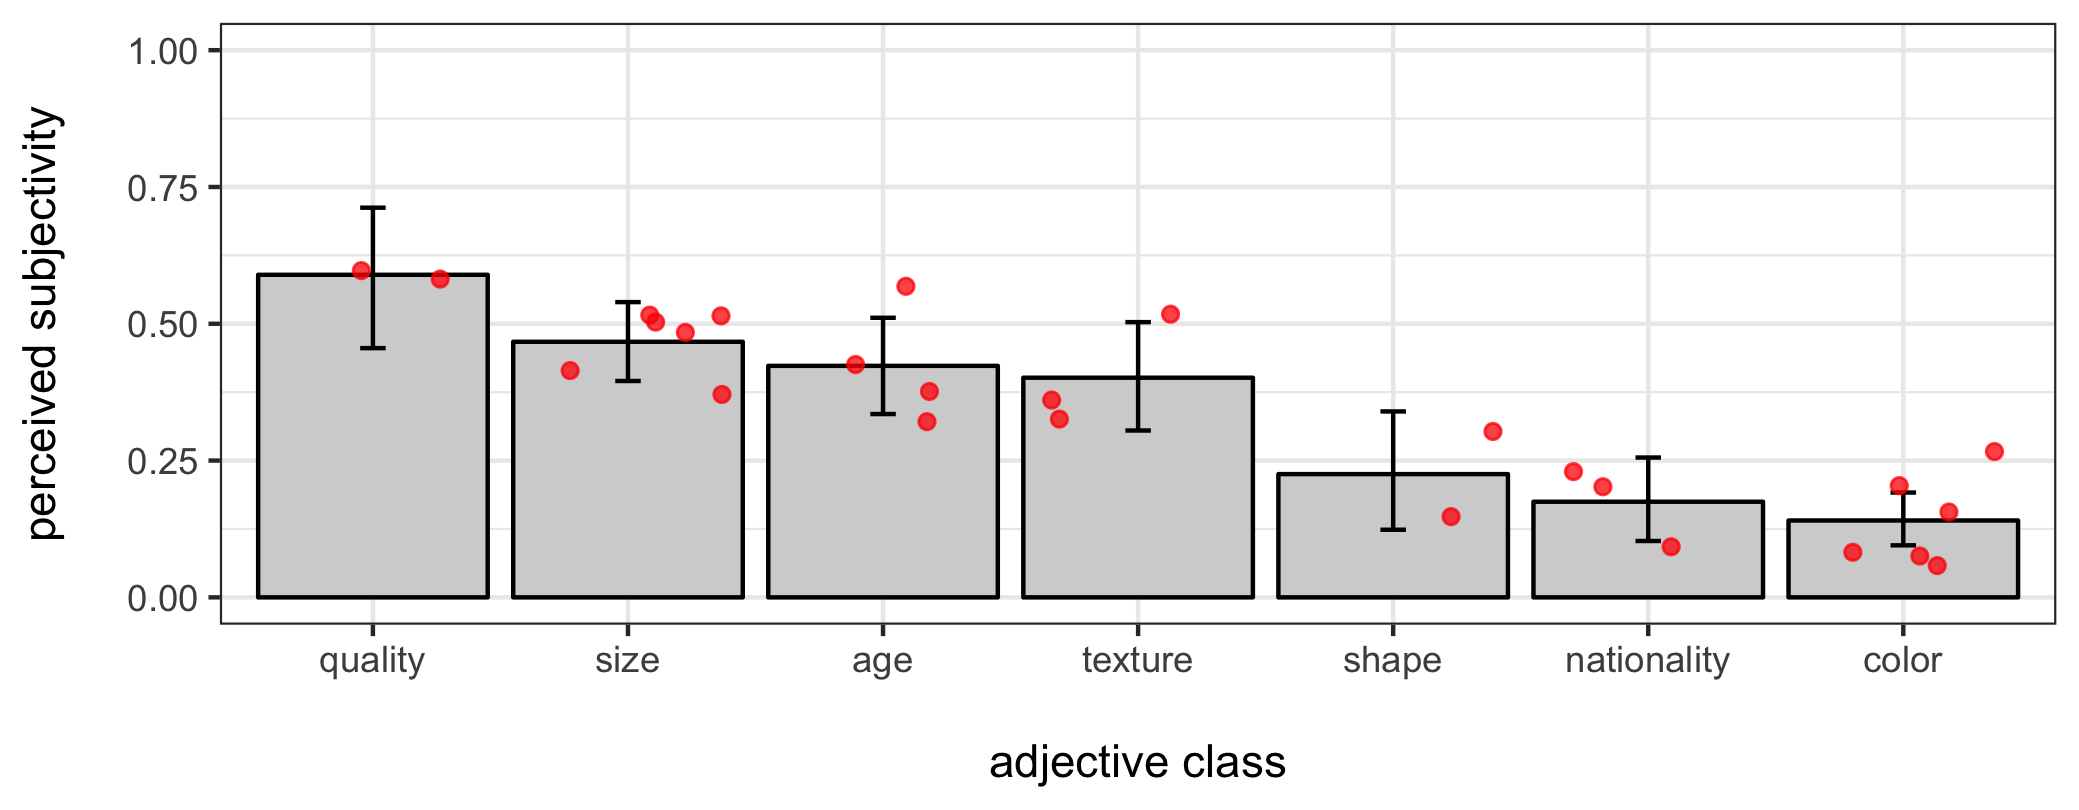
\includegraphics[height=2.5in]{class_subjectivity_jitter.eps}
	\caption{Faultless disagreement ratings from Experiment 1 grouped by adjective semantic class. Higher values indicate that a class's adjectives are more subjective. Error bars represent bootstrapped 95\% confidence intervals drawn from 10,000 samples of the data. Red dots represent point estimates for individual adjectives.
	}
	\label{exp2-results}
\end{figure}

For each adjective, we computed a mean perceived subjectivity score by averaging the faultless disagreement ratings across participants. Figure \ref{exp2-results} plots perceived subjectivity scores grouped by adjective class. Unlike with the ordering preferences, here we see that classes deviate from each other with respect to subjectivity. Below, we will use these scores to test the predictive power of subjectivity in the Spanish ordering preferences.

\subsection{Comparing ordering preferences with subjectivity}

\begin{figure}[t]
	\centering
	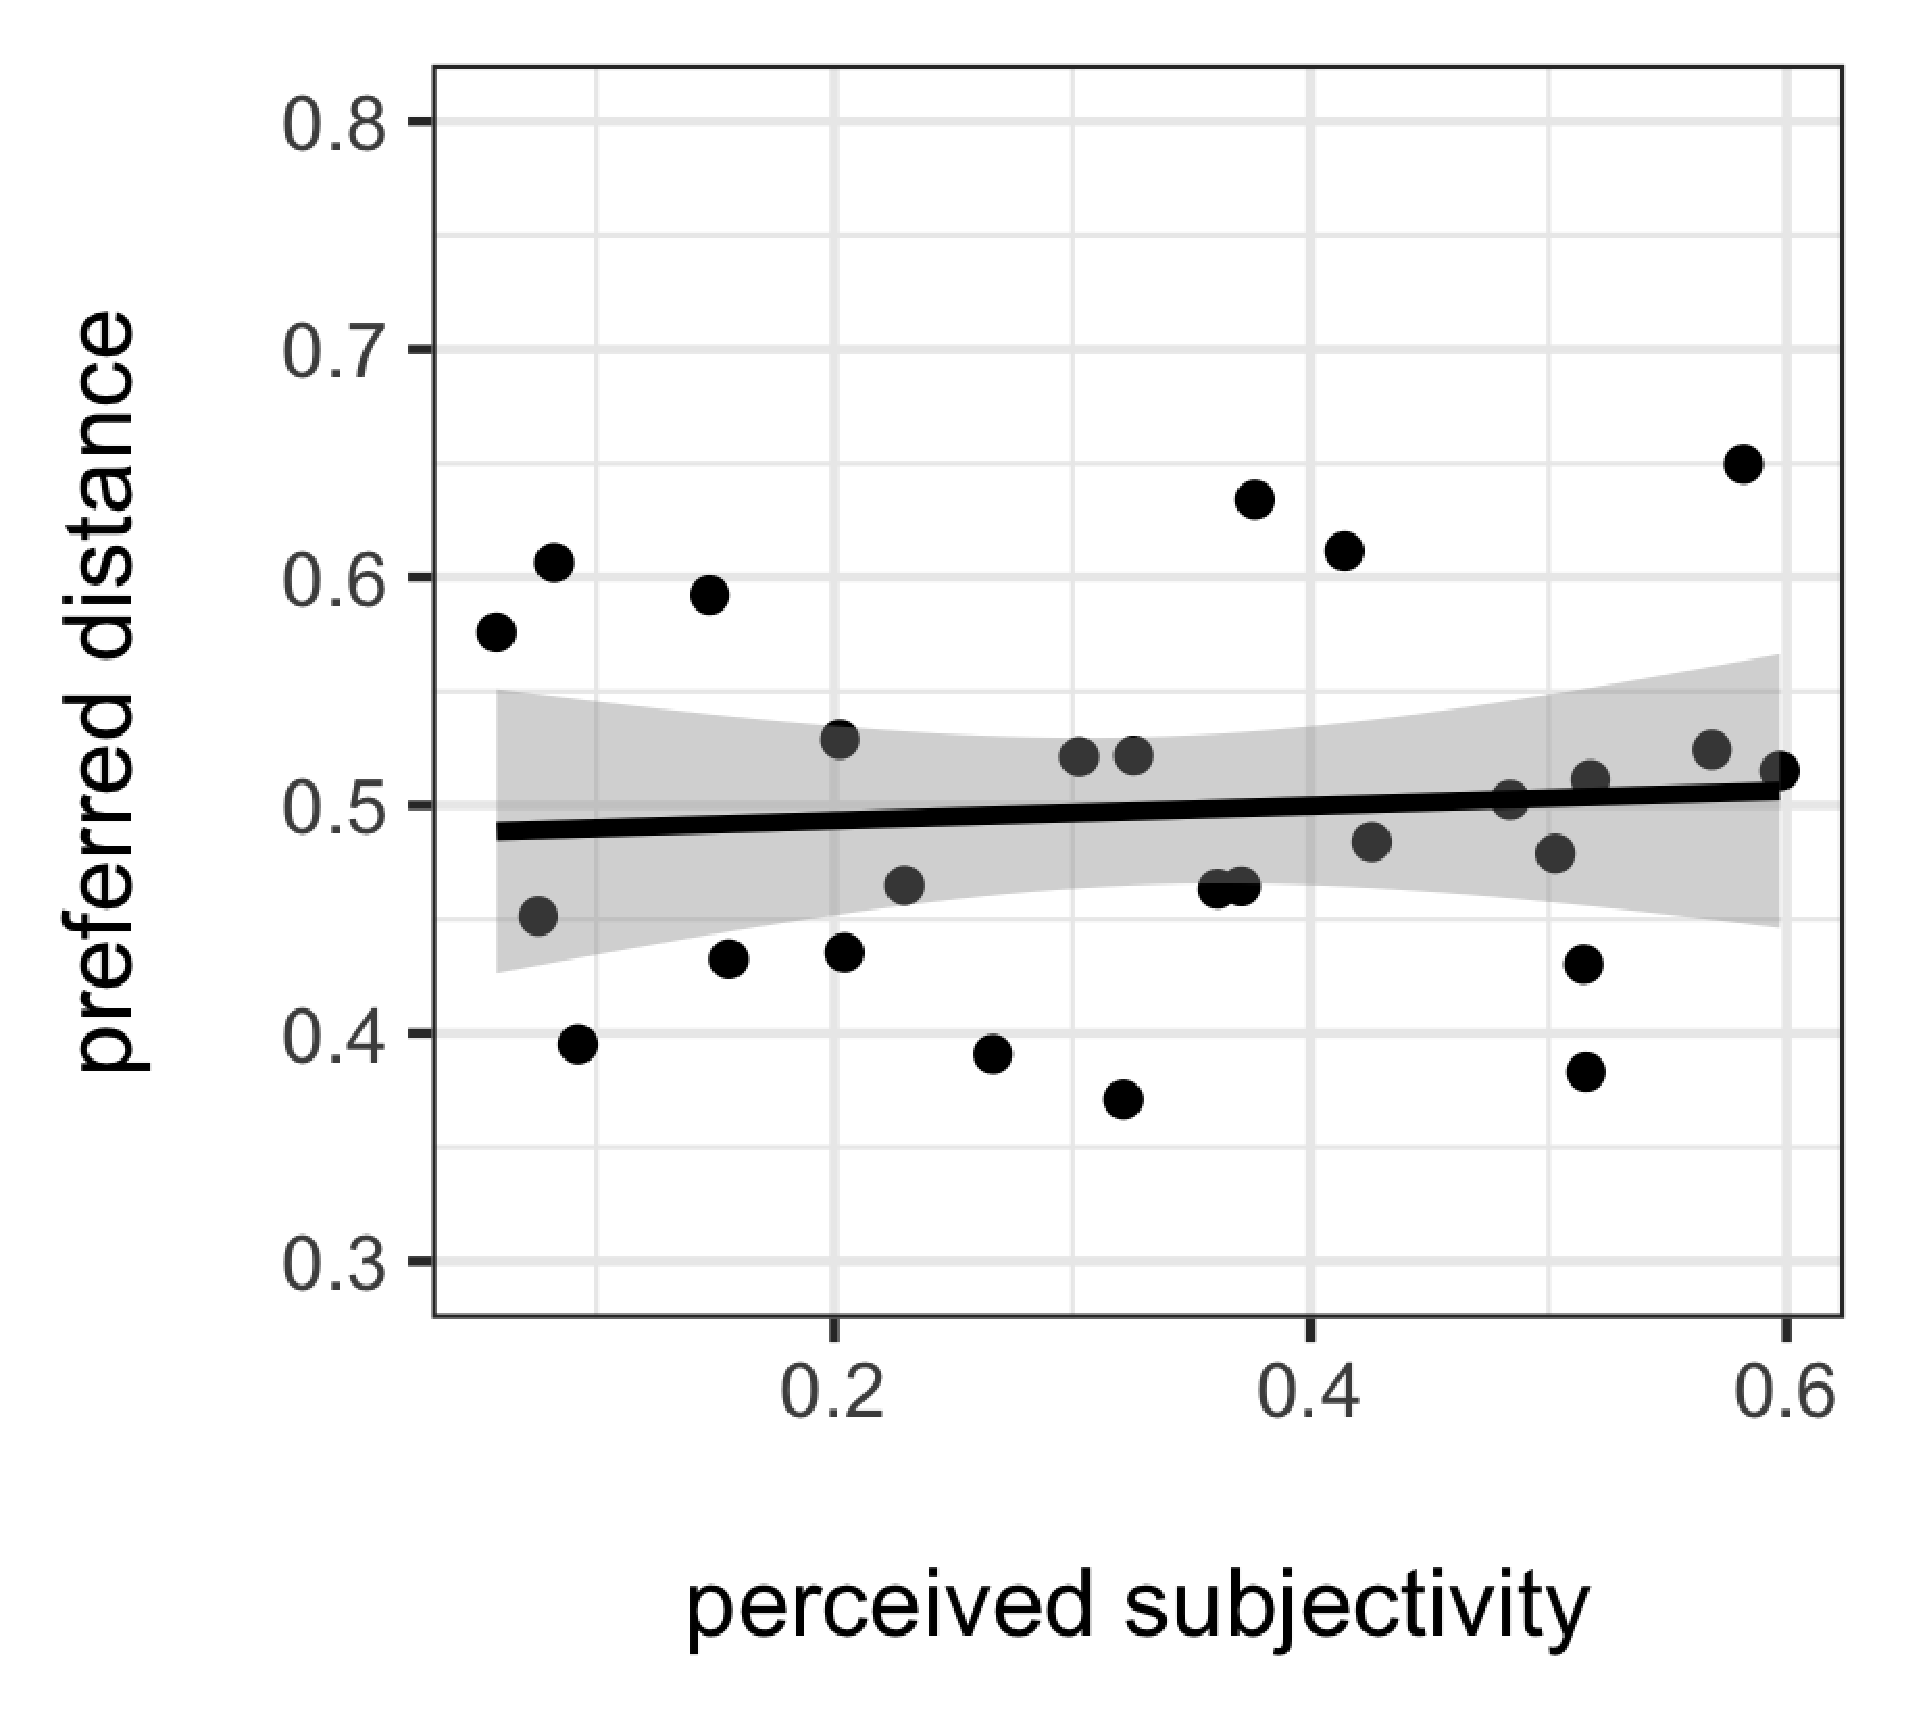
\includegraphics[height=2.5in]{naturalness-subjectivity-spanish-LSA-proceedings.eps}
	\caption{Spanish ordering preferences plotted against subjectivity scores for each of the 26 adjectives tested. %Subjectivity accounts for 54\% of the variance in the ordering preferences ($r^2$ = 0.54, 95\% CI = [0.22, 0.74]).
	}
	\label{subj-comparison}
\end{figure}

Finally, we compare the Spanish ordering preferences with perceived subjectivity to evaluate the extent to which subjectivity predicts adjective ordering preferences in Spanish. Figure \ref{subj-comparison} plots the ordering preferences against the subjectivity scores (i.e., faultless disagreement ratings) for each of the 26 adjectives. Adjective subjectivity accounts for 0.01\% of the variance in the ordering preferences ($r^2$ = 0.01; 95\% CI [0.00, 0.06]). In other words, subjectivity does not predict ordering preferences in Spanish, However, this finding is not a failure of subjectivity, but rather a byproduct of the absence of Spanish ordering preferences. As we would expect if ordering preferences arise from the hierarchical structure of nominal modification, when conjunction interrupts the incremental adjective composition, as in Spanish, ordering preferences do not arise. We follow up on this finding in the next section by testing the effect of conjunction on English ordering preferences.



\section{Experiment 2: English} \label{english}

Having failed to find ordering preferences in the presence of conjunction in Spanish, we turn next to English, where multi-adjective strings optionally feature conjunction. If we are on the right track in assuming that the pressure for subjectivity-based ordering preferences does not arise when conjunction interrupts the incremental semantic composition of multi-adjective modification, then we should find that conjunction neutralizes ordering preferences in Spanish, as it does in English. We therefore replicated the methodology of \emph{Expt.~1: Ordering preferences} from \cite{scontrasetal2017adjectives}, adding in a manipulation whereby some multi-adjective strings featured conjunction.

\subsection{Participants}


We recruited 60 participants through Amazon.com's Mechanical Turk. All participants were compensated for their participation. 59 participants identified as native speakers of English (41 female, 18 male; mean age: 36); their data were included in the analyses reported below.

\subsection{Procedure}

The design of this experiment was similar to that of \emph{Expt.~1: Ordering preferences} from \cite{scontrasetal2017adjectives}, with one crucial difference: the pairs of multi-adjective object descriptions that participants encountered appeared either with or without conjunction. For example, participants might judge the naturalness of \emph{big blue box} vs.~\emph{blue big box} (i.e., without conjunction), or they might see \emph{big and blue box} vs.~\emph{blue and big box} (i.e., with conjunction). Participants completed a total of 26 trials. For each object description, adjectives and nouns were chosen at random and came from the original English materials from \cite{scontrasetal2017adjectives}; whether or not the description featured conjunction was chosen at random on each trial.

\subsection{Results}

\begin{figure}
	\centering
	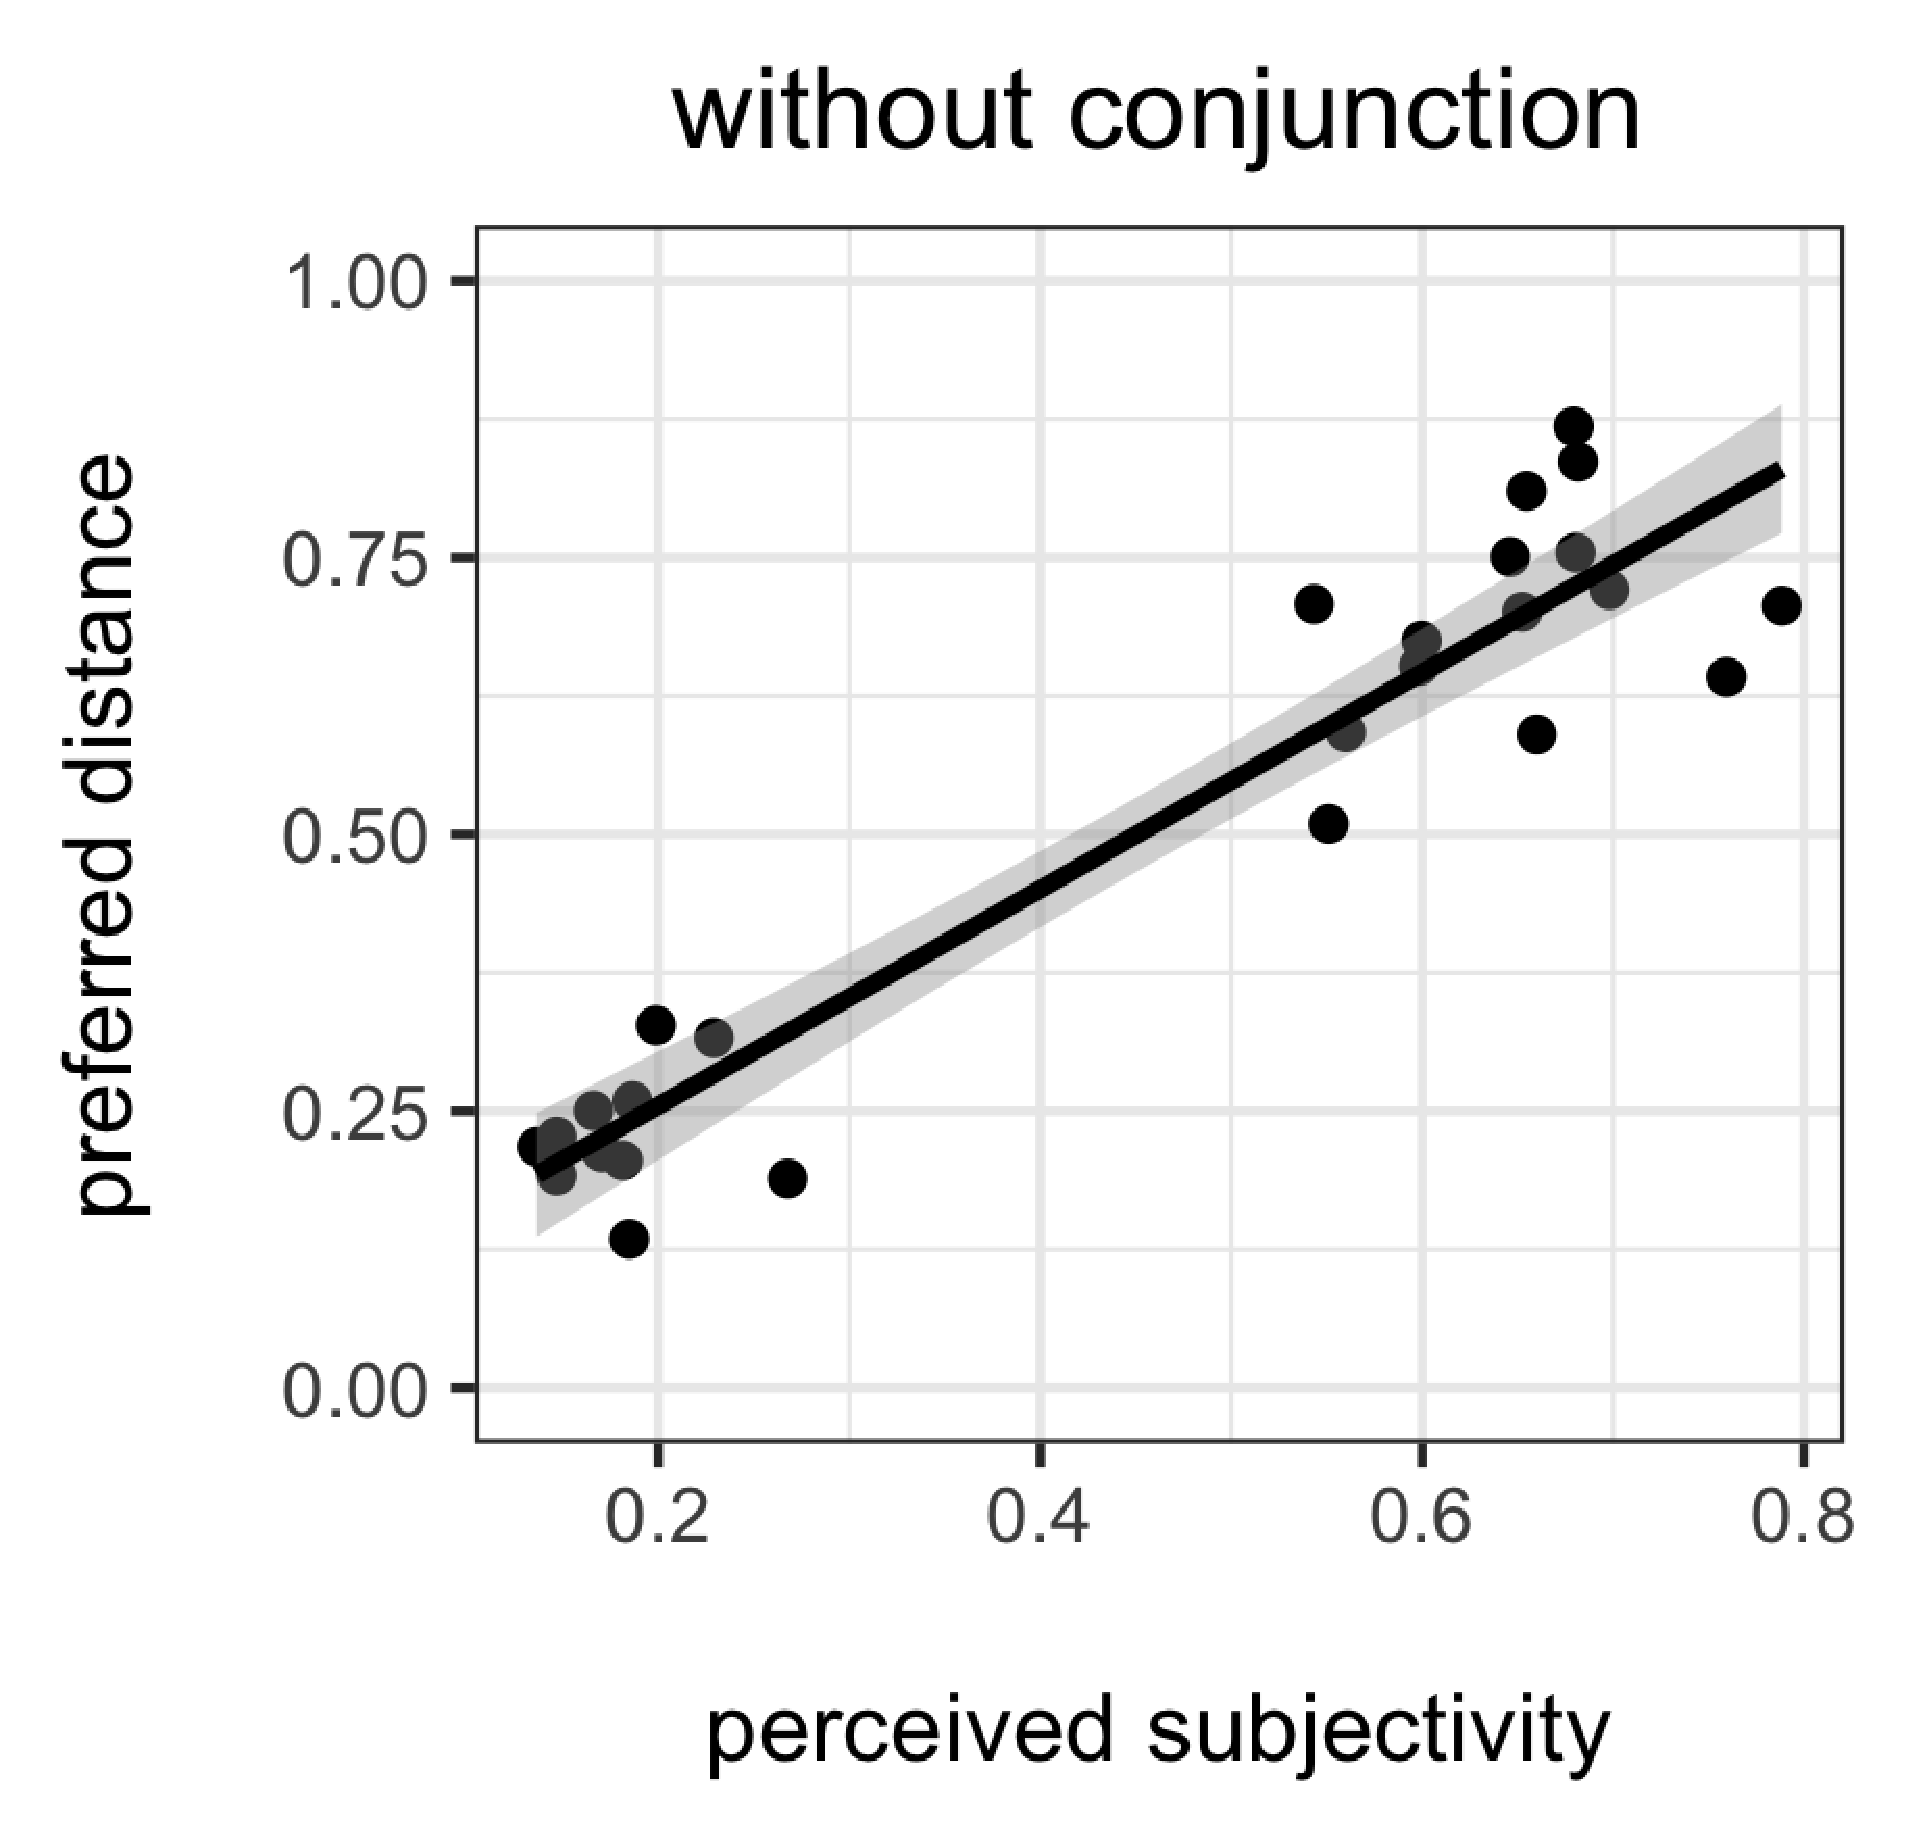
\includegraphics[height=2.5in]{naturalness-subjectivity-NOconjunction-LSA.eps}		
	\quad \quad \quad
	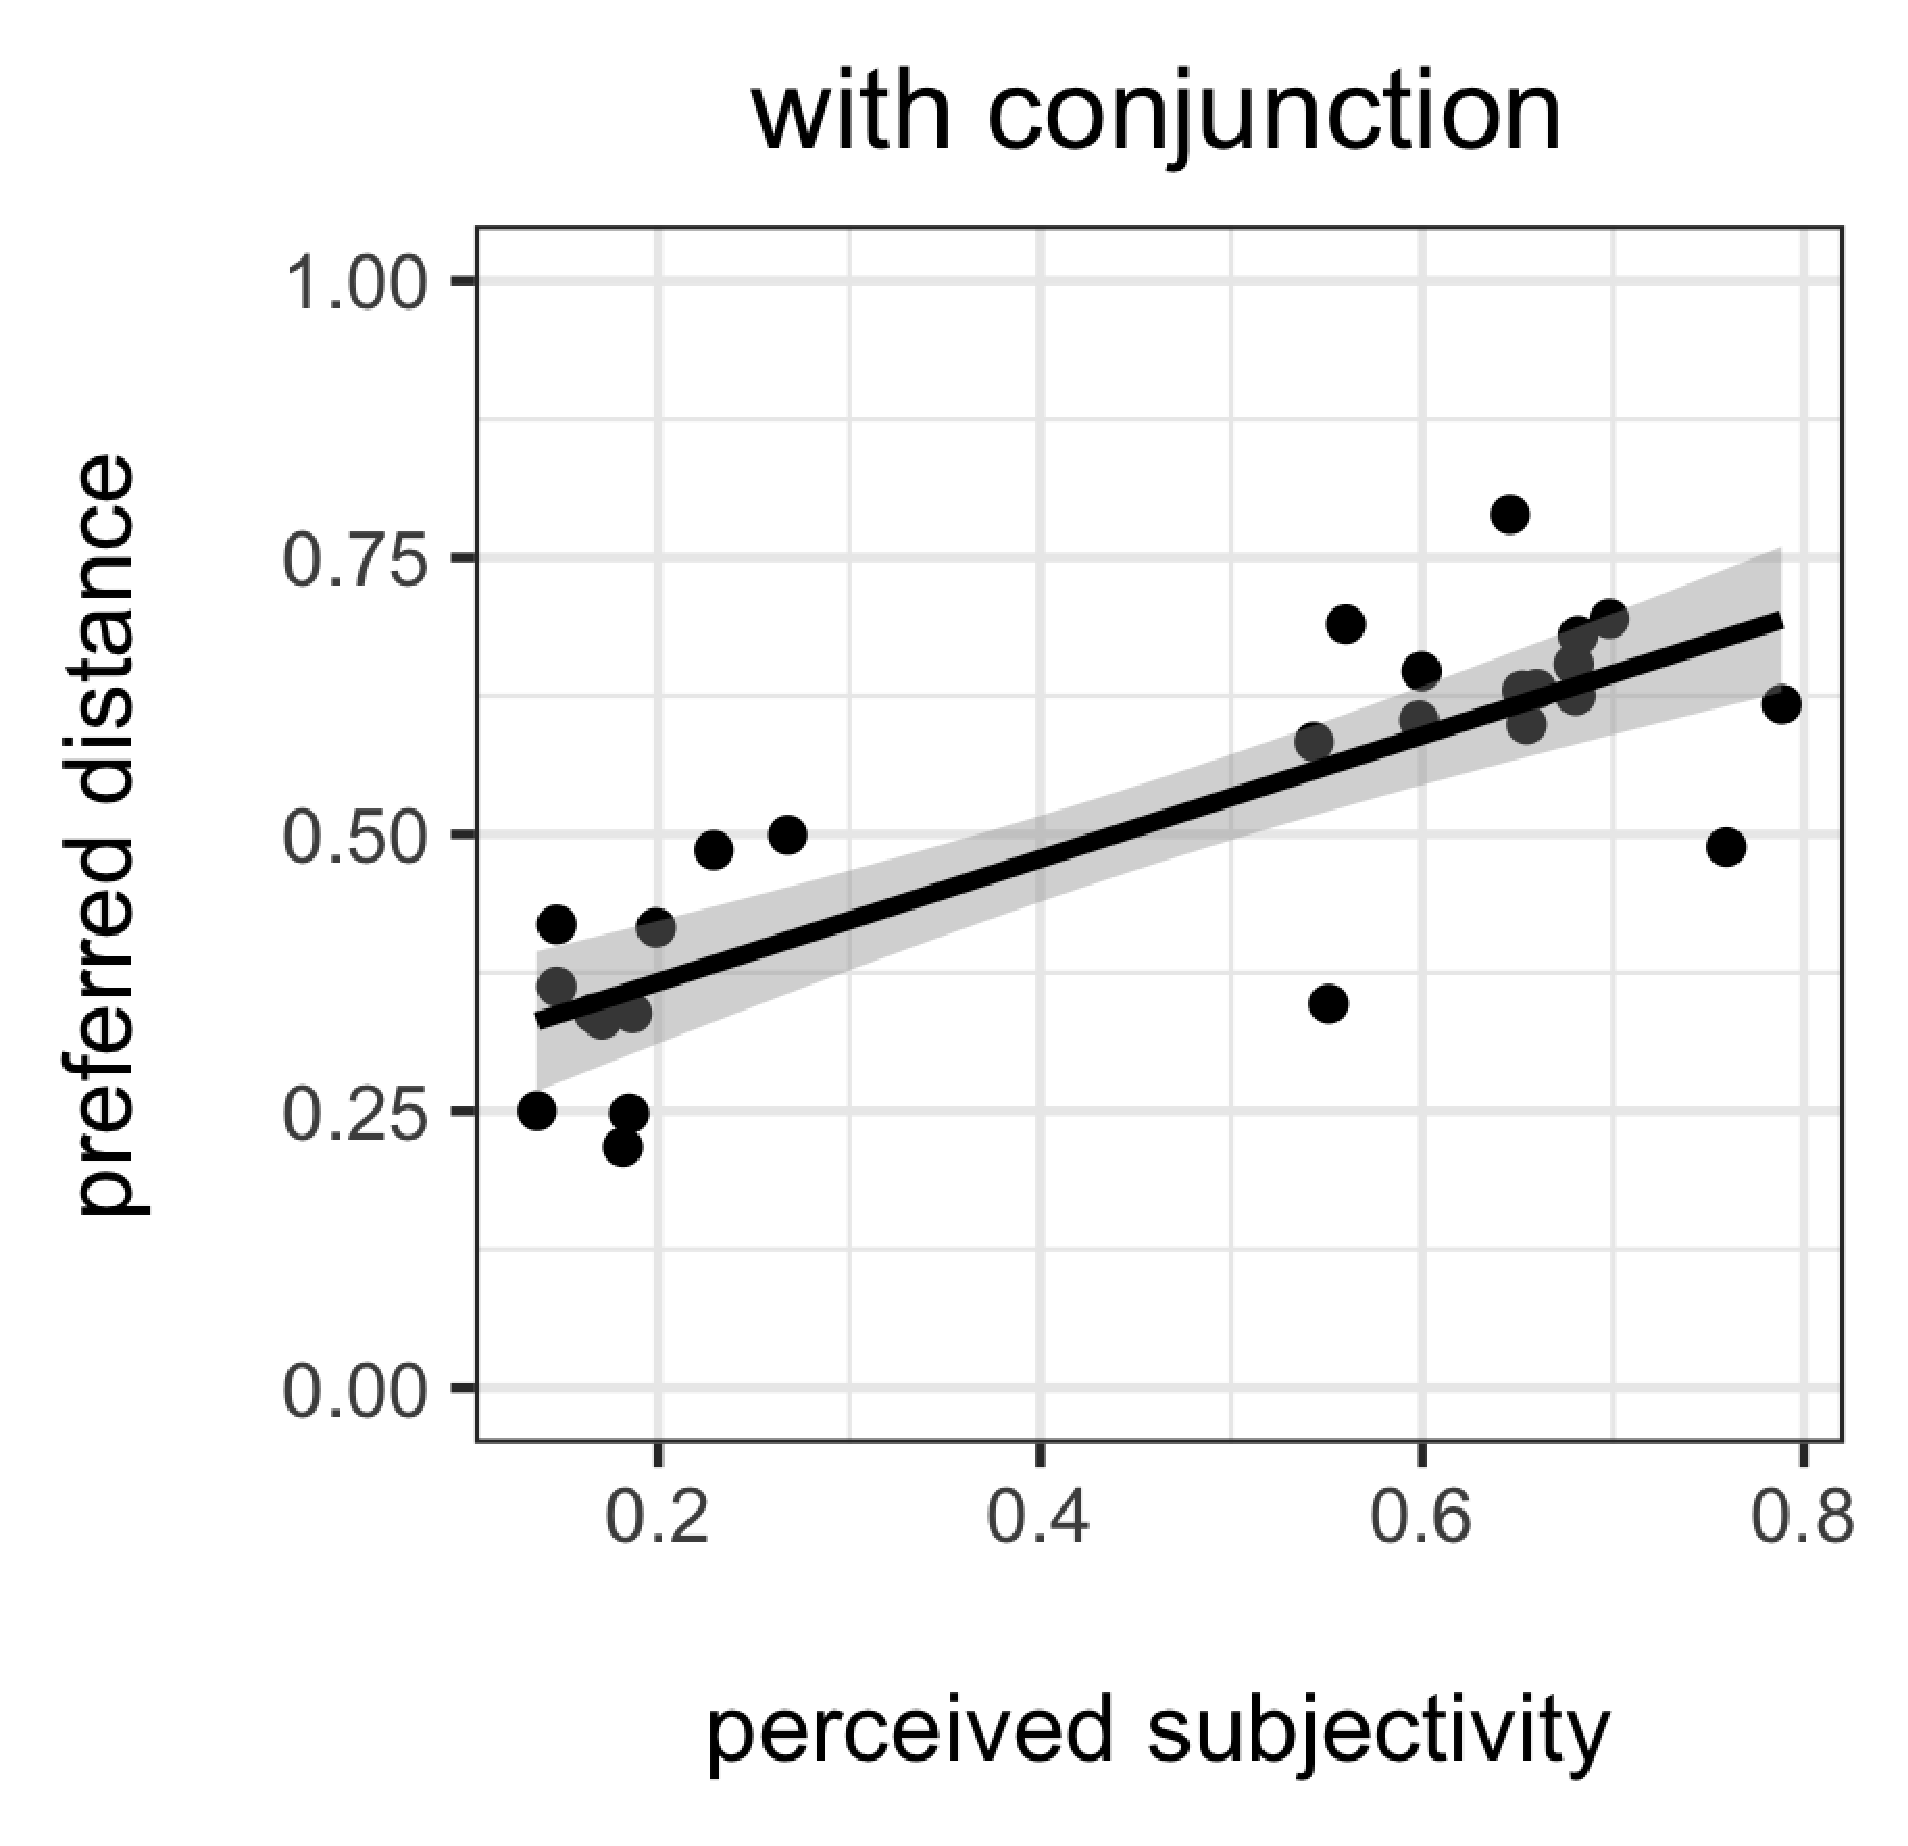
\includegraphics[height=2.5in]{naturalness-subjectivity-conjunction.eps}
	\caption{English ordering preferences both with (\emph{right}) and without (\emph{left}) conjunction plotted against subjectivity scores for each of the 26 adjectives tested. %Subjectivity accounts for 54\% of the variance in the ordering preferences ($r^2$ = 0.54, 95\% CI = [0.22, 0.74]).
	}
	\label{english-subj-comparison}
\end{figure}

As with the Spanish ordering preferences, we calculated a mean preferred-distance measure both with and without conjunction by averaging across participants. Figure \ref{english-subj-comparison} plots these preferred distance measures against the English adjective subjectivity scores from \cite{scontrasetal2017adjectives}. As expected, subjectivity accounts for nearly all of the variance in multi-adjective strings without conjunction ($r^2$ = 0.89; 95\% CI [0.81, 0.94])---this result replicates the original findings of \cite{scontrasetal2017adjectives}. What comes as a surprise, however, is the presence of subjectivity-based ordering preferences \emph{with} conjunction: although the effect is weaker with conjunction, subjectivity continues to predict ordering preferences ($r^2$ = 0.68; 95\% CI [0.40, 0.83]). This finding stands in stark contrast to the Spanish results, where subjectivity accounted for next to no variance in the ordering preferences. In other words, in the presence of conjunction, subjectivity-based ordering preferences weaken but persist in English.




\section{General discussion} \label{discussion}

We have found mixed results on the status of subjectivity-based ordering preferences in the presence of conjunction. In Spanish, where multi-adjective strings are post-nominal and require conjunction, we failed to find evidence of stable ordering preferences, subjectivity-based or otherwise. In English, where multi-adjective strings optionally feature conjunction, we found that with conjunction subjectivity-based ordering preferences weaken but persist. This result is surprising in light of previous claims regarding the role of conjunction in English ordering preferences. Returning to the explanations for subjectivity-based preferences discussed in Section \ref{background}, the hierarchical accounts of \cite{simonic2018} and \cite{scontrasetalSPadjectives} straightforwardly predict the Spanish findings: conjunction interrupts the incremental hierarchical composition, such that adjectives farther from the noun no longer classify a smaller set out potential referents. Without incremental restriction, the pressures for subjectivity-based orderings are no longer present, thereby accounting for the lack of preferences in Spanish.

However, the story we have just told applies also to cases of conjunction in English, but in English we continue to find stable subjectivity-based preferences in the presence of conjunction. Either we are wrong about our explanation for the absence of stable preference in Spanish, or some other factor delivers the observed preferences in English. We begin by pursuing the first option. In addition to requiring conjunction, another feature separates the Spanish multi-adjective strings from their English cousins: in Spanish, multi-adjective strings are post-nominal, following the modified noun. Perhaps this feature is responsible for the absence of stable preferences in Spanish. However, \cite{Martin1969competence} documented stable ordering preferences in Indonesian, a language with post-nominal adjectives. Moreover, the preferences \citeauthor{Martin1969competence} documented matched those found in English, suggesting that Indonesian has subjectivity-based preferences as well. Crucially, while Indonesian has post-nominal adjectives, it does not require conjunction to form its multi-adjective strings. Thus, we find it unlikely that post-nominal adjectives are to blame for the absence of stable preference in Spanish; conjunction appears to be the culprit, and the hierarchical explanations of \citeauthor{simonic2018} and \citeauthor{scontrasetalSPadjectives}~offer an explanation for why.

But why then should preferences persist in the presence of conjunction in English? Here we are limited to speculation, but there appears to be a viable lead to pursue. Spanish and English differ in that Spanish requires conjunction in multi-adjective strings, whereas in English conjunction is optional. This optionality means that speakers of English will encounter many multi-adjective strings without conjunction, where pressures toward subjectivity-based orderings apply. In other words, the regularity introduced by subjectivity-based preferences is present already in English, such that this regularity can be extended by analogy to cases with conjunction. Here a laundry metaphor seems rather apt: if one washes some white and clean sheets (conjunction) with dirty red socks (no conjunction), the sheets will come out a little pinker after the wash. The regularity present in the conjunction-free cases bleeds over into the cases with conjunction. In Spanish, where multi-adjective strings require conjunction, there is no source for the regularity that could bleed over into in the cases with conjunction.

That the English ordering preferences in conjoined multi-adjective strings should find their source in the conjunction-free strings suggests that the preferences do not arise from active, rational reasoning processes from speakers. Rather, these preferences are more likely to arise via an evolutionary process whereby speakers attend to communicative success in the conjunction-free strings, and the regularity that results gets extended by analogy to the conjoined strings. Returning to the predictions we set out to test, our results support the hierarchical explanations of communicative success: with conjunction, pressures for subjectivity-based orderings do not arise so long as the language does not have some other source for ordering regularities. \\[15pt]
%There is another possibility. Perhaps both linear and hierarchical pressures do apply 
 
% ------------ references --------------------------------------------------------------------------------------
\setlength{\bibsep}{0pt plus 0.3ex}
\setlength{\bibhang}{0.3in}			% hanging indent for references must be 0.3in
\titleformat{\section}{\normalfont\bfseries}{\thesection}{.5em}{}		% references section not supposed to be followed by a period


\bibliographystyle{sp.bst}		% S\&P bibliography style
%S\&P, an LSA publication, meets the LSA guidelines. 
%See: http://info.semprag.org 
%and get the bst at: https://raw.githubusercontent.com/semprag/tex/master/sp.bst 
%If using the sp.bst, the following command turns your DOIs into links
\newcommand{\doi}[1]{\href{http://dx.doi.org/#1}{http://dx.doi.org/#1}}	%modified from sp.cls
\bibliography{greg}			% your bib file

\end{document}
 
 
 
 